\documentclass[12pt]{article}
%\usepackage[backend=biber]{biblatex}
\usepackage{amsmath}
\usepackage{listings}
\usepackage{graphicx}
\usepackage{caption}
\usepackage{subcaption}
\usepackage{commath}
\usepackage{hyperref}
\usepackage{url}
\usepackage{xcolor}
\usepackage{textcomp}
\usepackage{dirtytalk}
\usepackage{listings}
\usepackage{wasysym}
\usepackage{float}
\usepackage{listings}
\usepackage[linesnumbered,lined,boxed,commentsnumbered]{algorithm2e}

% Packages from derivations_fullproblem.tex
\usepackage[squaren]{SIunits}
\usepackage{a4wide}
\usepackage{array}
\usepackage{cancel}
\usepackage{amsmath}
\usepackage{amsfonts}
\usepackage{amssymb}
\usepackage{graphicx}
\usepackage{enumerate}

% Parameters for displaying code.
\lstset{language=C++}
\lstset{basicstyle=\ttfamily\small}
\lstset{frame=single}
\lstset{keywordstyle=\color{red}\bfseries}
\lstset{commentstyle=\itshape\color{blue}}
\lstset{showspaces=false}
\lstset{showstringspaces=false}
\lstset{showtabs=false}
\lstset{breaklines}

% Define new commands
\newcommand{\expect}[1]{\langle #1 \rangle}

% Add bibliography
\begin{document}


\title{MAT4110 - Oblig 2}
\author{Geir Tore Ulvik - ulvik}
\maketitle

\section{Introduction}
In this work, compression of grayscale images using Singular Value
Decomposition (SVD) is studied. Three images are used: 
\begin{itemize}
	\item \href{https://pixabay.com/en/board-chess-chessboard-black-white-157165/}{A chessboard}
	\item \href{https://pixabay.com/en/jellyfish-under-water-sea-ocean-698521/}{A submerged jellyfish}
	\item \href{https://pixabay.com/en/new-york-city-skyline-nyc-690868/}{An image of New York}
\end{itemize}
When applying SVD to an $n\times m$ matrix, a number of the singular values
will have a very small contribution to the reconstruction of the original
matrix. These singular values can be removed, effectively discarding 
information from the images that isn't very important.
The compression ratio
\begin{equation}
	\text{compression ratio} = \frac{\text{original size}}{\text{compressed size}}
\end{equation}
is studied as a function of $n$, $m$, and $r$, where $r$ is the number of
singular values kept.
The code used to produce the results and plots is available on GitHub:\\ 
\url{https://github.com/geirtul/mat4110/blob/master/oblig2/analysis.py}
\section{Results and Discussion}
Figure \ref{fig:comp-r} shows how the compression ratio for the three images
varies when varying $r > 5$. Below these values the compression follows the
same trend, but for the chessboard it rises far more sharply than for the
other images. This is to be expected, since the chessboard image is
essentially just $8\times 8$ pixels, even though the images has a higher
resolution than that.

For the other two images it seems the compression ratio will approach
that of the chessboard as $r$ approaches the total number of singular
values. This is also expected, as a compression ratio of 1 indicates
no compression.

Looking at the compression ratio as a function of $n$ and $m$, in
figure \ref{fig:comp-nm} we see that the general trend is that it
increases when reducing the number of colums or rows.
However, for the jellyfish and new york images, the ratio decreases for the
first $~200$, before it follows the same trend and the rest. The reason
for this is not known, but it could be an implementation error.

A compressed version of each image is presented along with its original
(in grayscale) in figures 
\ref{fig:comparison-chess}, \ref{fig:comparison-jelly}, \ref{fig:comparison-ny}.

\section{Figures}
\begin{figure}[h]
	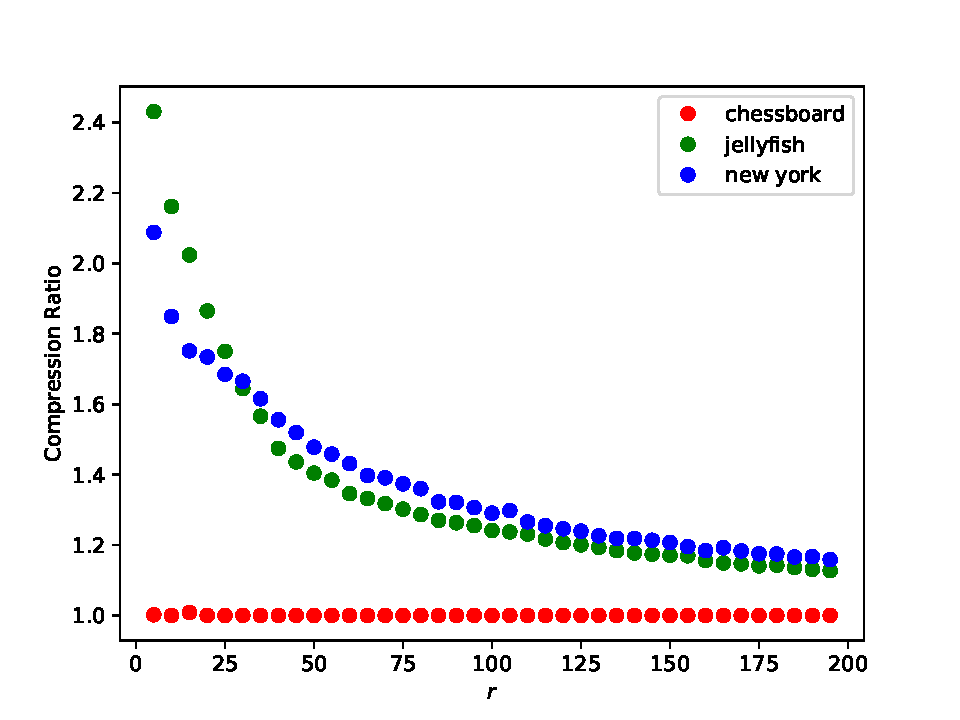
\includegraphics[width = \textwidth]{figures/compression_ratio_r.pdf}
	\caption{Compression ratio as a function of the number of singular
	values $r > 5$ kept. Values of $r$ lower than 5 kept out for 
	esthetic reasons.}
	\label{fig:comp-r}
\end{figure}
\begin{figure}[h]
	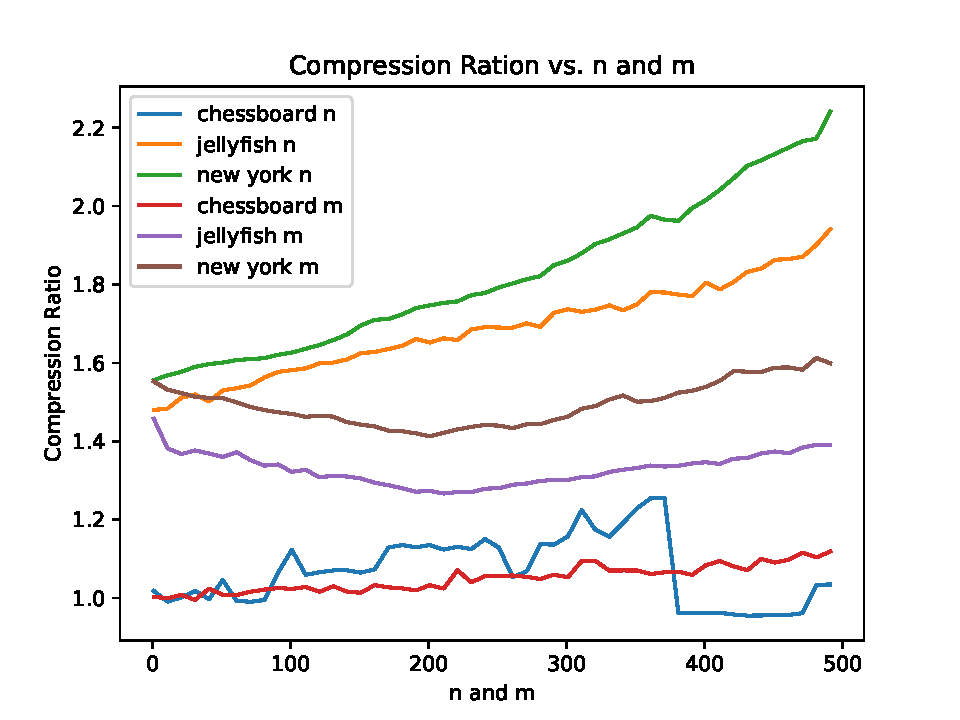
\includegraphics[width = \textwidth]{figures/compression_ratio_nm.pdf}
	\caption{Compression ratio as a function of $n$ and $m$. Increasing $n$ and $m$ corresponds to removing $n$ rows or $m$ columns from the image before compression with SVD. $r = const. = 40$.}
	\label{fig:comp-nm}
\end{figure}

\begin{figure}[h]
	\begin{align*}
		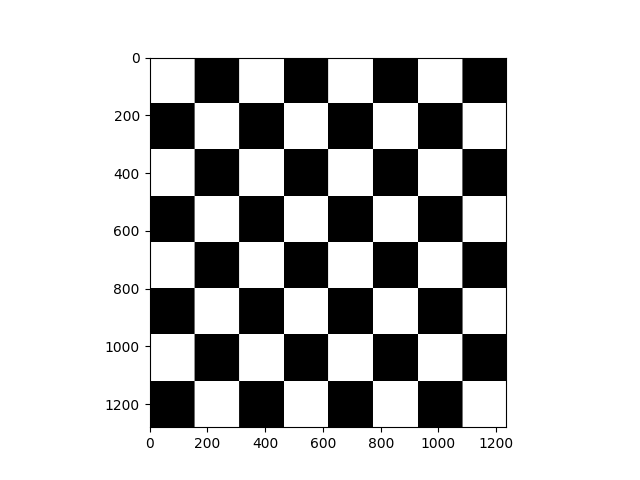
\includegraphics[width = 0.8\textwidth]{figures/chessboard_compressed} \\
		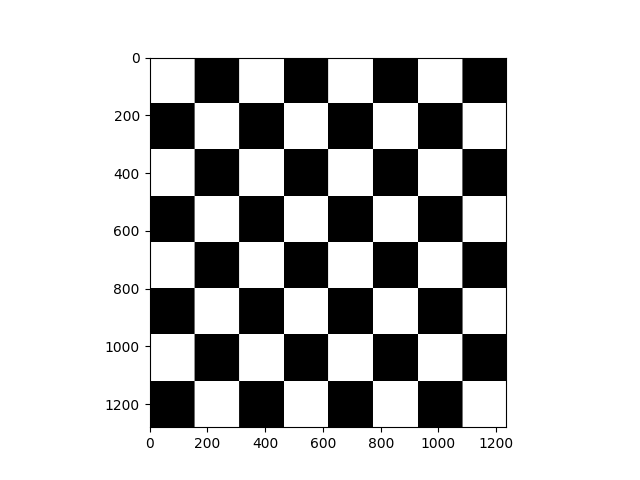
\includegraphics[width = 0.8\textwidth]{figures/chessboard_noncompressed}
	\end{align*}
	\caption{Comparison of the compressed (top) and uncompressed 
	(bottom) chessboard image. The images were both output in the 
	png format in grayscale. $r = 20$.}
	\label{fig:comparison-chess}
\end{figure}
\begin{figure}[h]
	\begin{align*}
		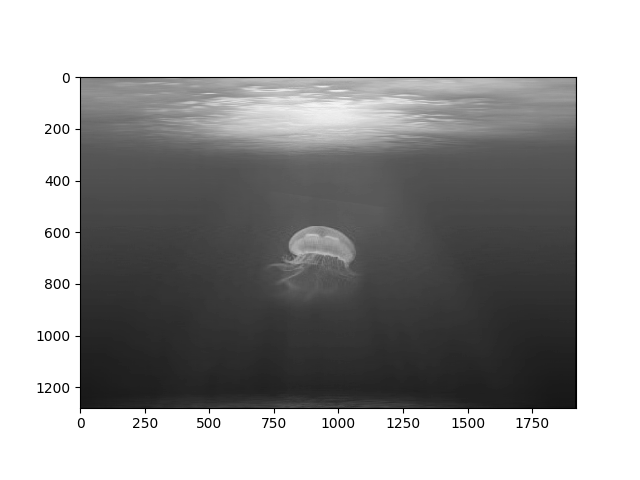
\includegraphics[width = 0.8\textwidth]{figures/jellyfish_compressed} \\
		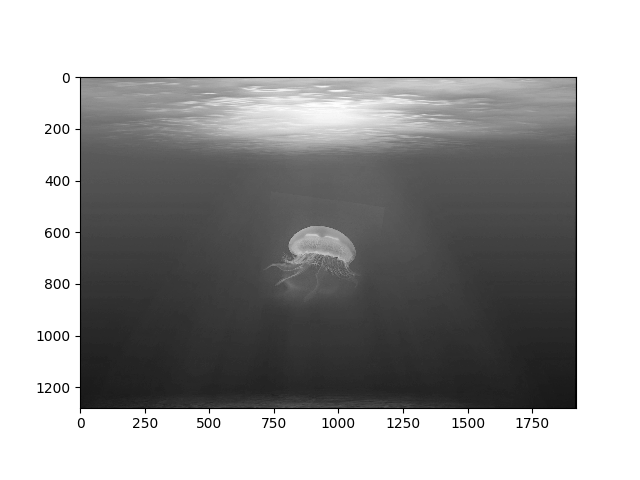
\includegraphics[width = 0.8\textwidth]{figures/jellyfish_noncompressed}
	\end{align*}
	\caption{Comparison of the compressed (top) and uncompressed 
	(bottom) jellyfish image. The images were both output in the 
	png format in grayscale.$r=50$}
	\label{fig:comparison-jelly}
\end{figure}
\begin{figure}[h]
	\begin{align*}
		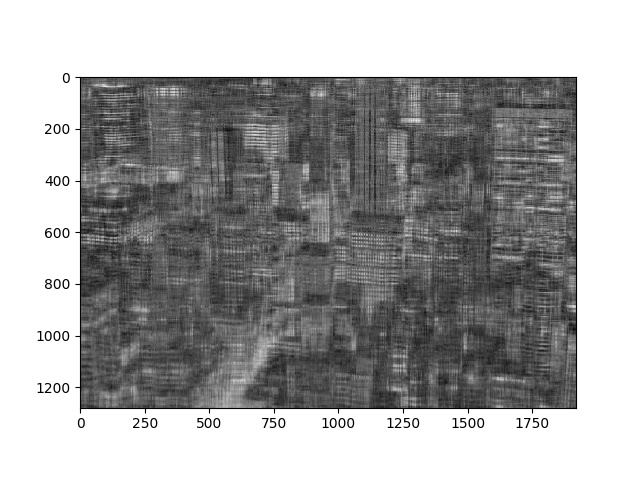
\includegraphics[width = 0.8\textwidth]{figures/new_york_compressed} \\
		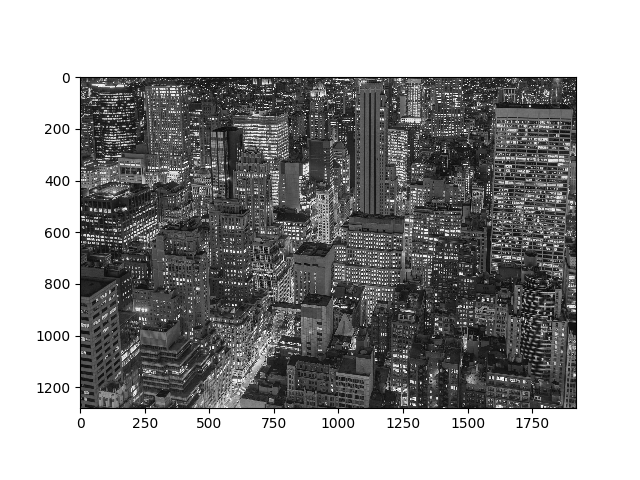
\includegraphics[width = 0.8\textwidth]{figures/new_york_noncompressed}
	\end{align*}
	\caption{Comparison of the compressed (top) and uncompressed 
	(bottom) jellyfish image. The images were both output in the 
	png format in grayscale. $r=100$}
	\label{fig:comparison-ny}
\end{figure}

\end{document}
